\documentclass[12pt,a4paper,oneside]{article} % part, *section, *paragraph
%\documentclass[12pt,a4paper,oneside]{report} % part, *chapter, *section, *paragraph
%\documentclass[12pt,a4paper,oneside]{book} % part, *chapter, *section, *paragraph

\usepackage[english]{babel}
\usepackage[latin2]{inputenc}
\usepackage{setspace}
\usepackage{float}
\usepackage[T1]{fontenc} %\showhyphens{integetnem} \showhyphens{meggy�ltetv�ny}
%\usepackage{ucs}\usepackage[utf8x]{inputenc}
%\usepackage{fullpage} %\usepackage[margin=2cm]{geometry}
%\usepackage{amsmath,amssymb}
\usepackage{url} %VAGY %\usepackage[unicode]{hyperref}
%\usepackage{listings} % forr�sk�dhoz
%\usepackage{color} 
\usepackage{graphicx}
\usepackage{times}
\usepackage{fullpage}
%\usepackage{showkeys} % \label{} ki�r�sa \ref{}hez
 
%\let\stdsection\section
%\renewcommand\section{\clearpage\stdsection}
\begin{document}
\onehalfspacing
\begin{center}
\vspace{2em}
%\large{\bf{}BUDAPESTI M\H{U}SZAKI \'ES GAZDAS\'AGTUDOM\'ANYI EGYETEM}
\vspace{.5em}


\includegraphics[width=60mm]{10000000000004C00000014A5D3CE278.eps}

Budapest University of Technology and Economics

Department of Measurement and Information Systems
%\vspace{.5em}

%\large{\bf{}VILLAMOSM\'ERN\"OKI \'ES INFORMATIKAI KAR\\
%M\'ERN\"OK INFORMATIKUS SZAK}

\vspace{2em}

%\Large{Informatikai Technol\'ogi\'ak szakir\'any\\
%Rendszerfejleszt\'es \'agazat}

%\vspace{1.5em}

%\Large{\bf{}\"On\'all\'o labor (BMEVIIIA337)}

%\vspace{1.5em}

\LARGE{\bf{}Fault tolerance and performance of dm-mirror}

\vspace{2em}

\begin{tabular}{ l c}
  %hopefully i can avoid the photo this time
  %\parbox{30mm}{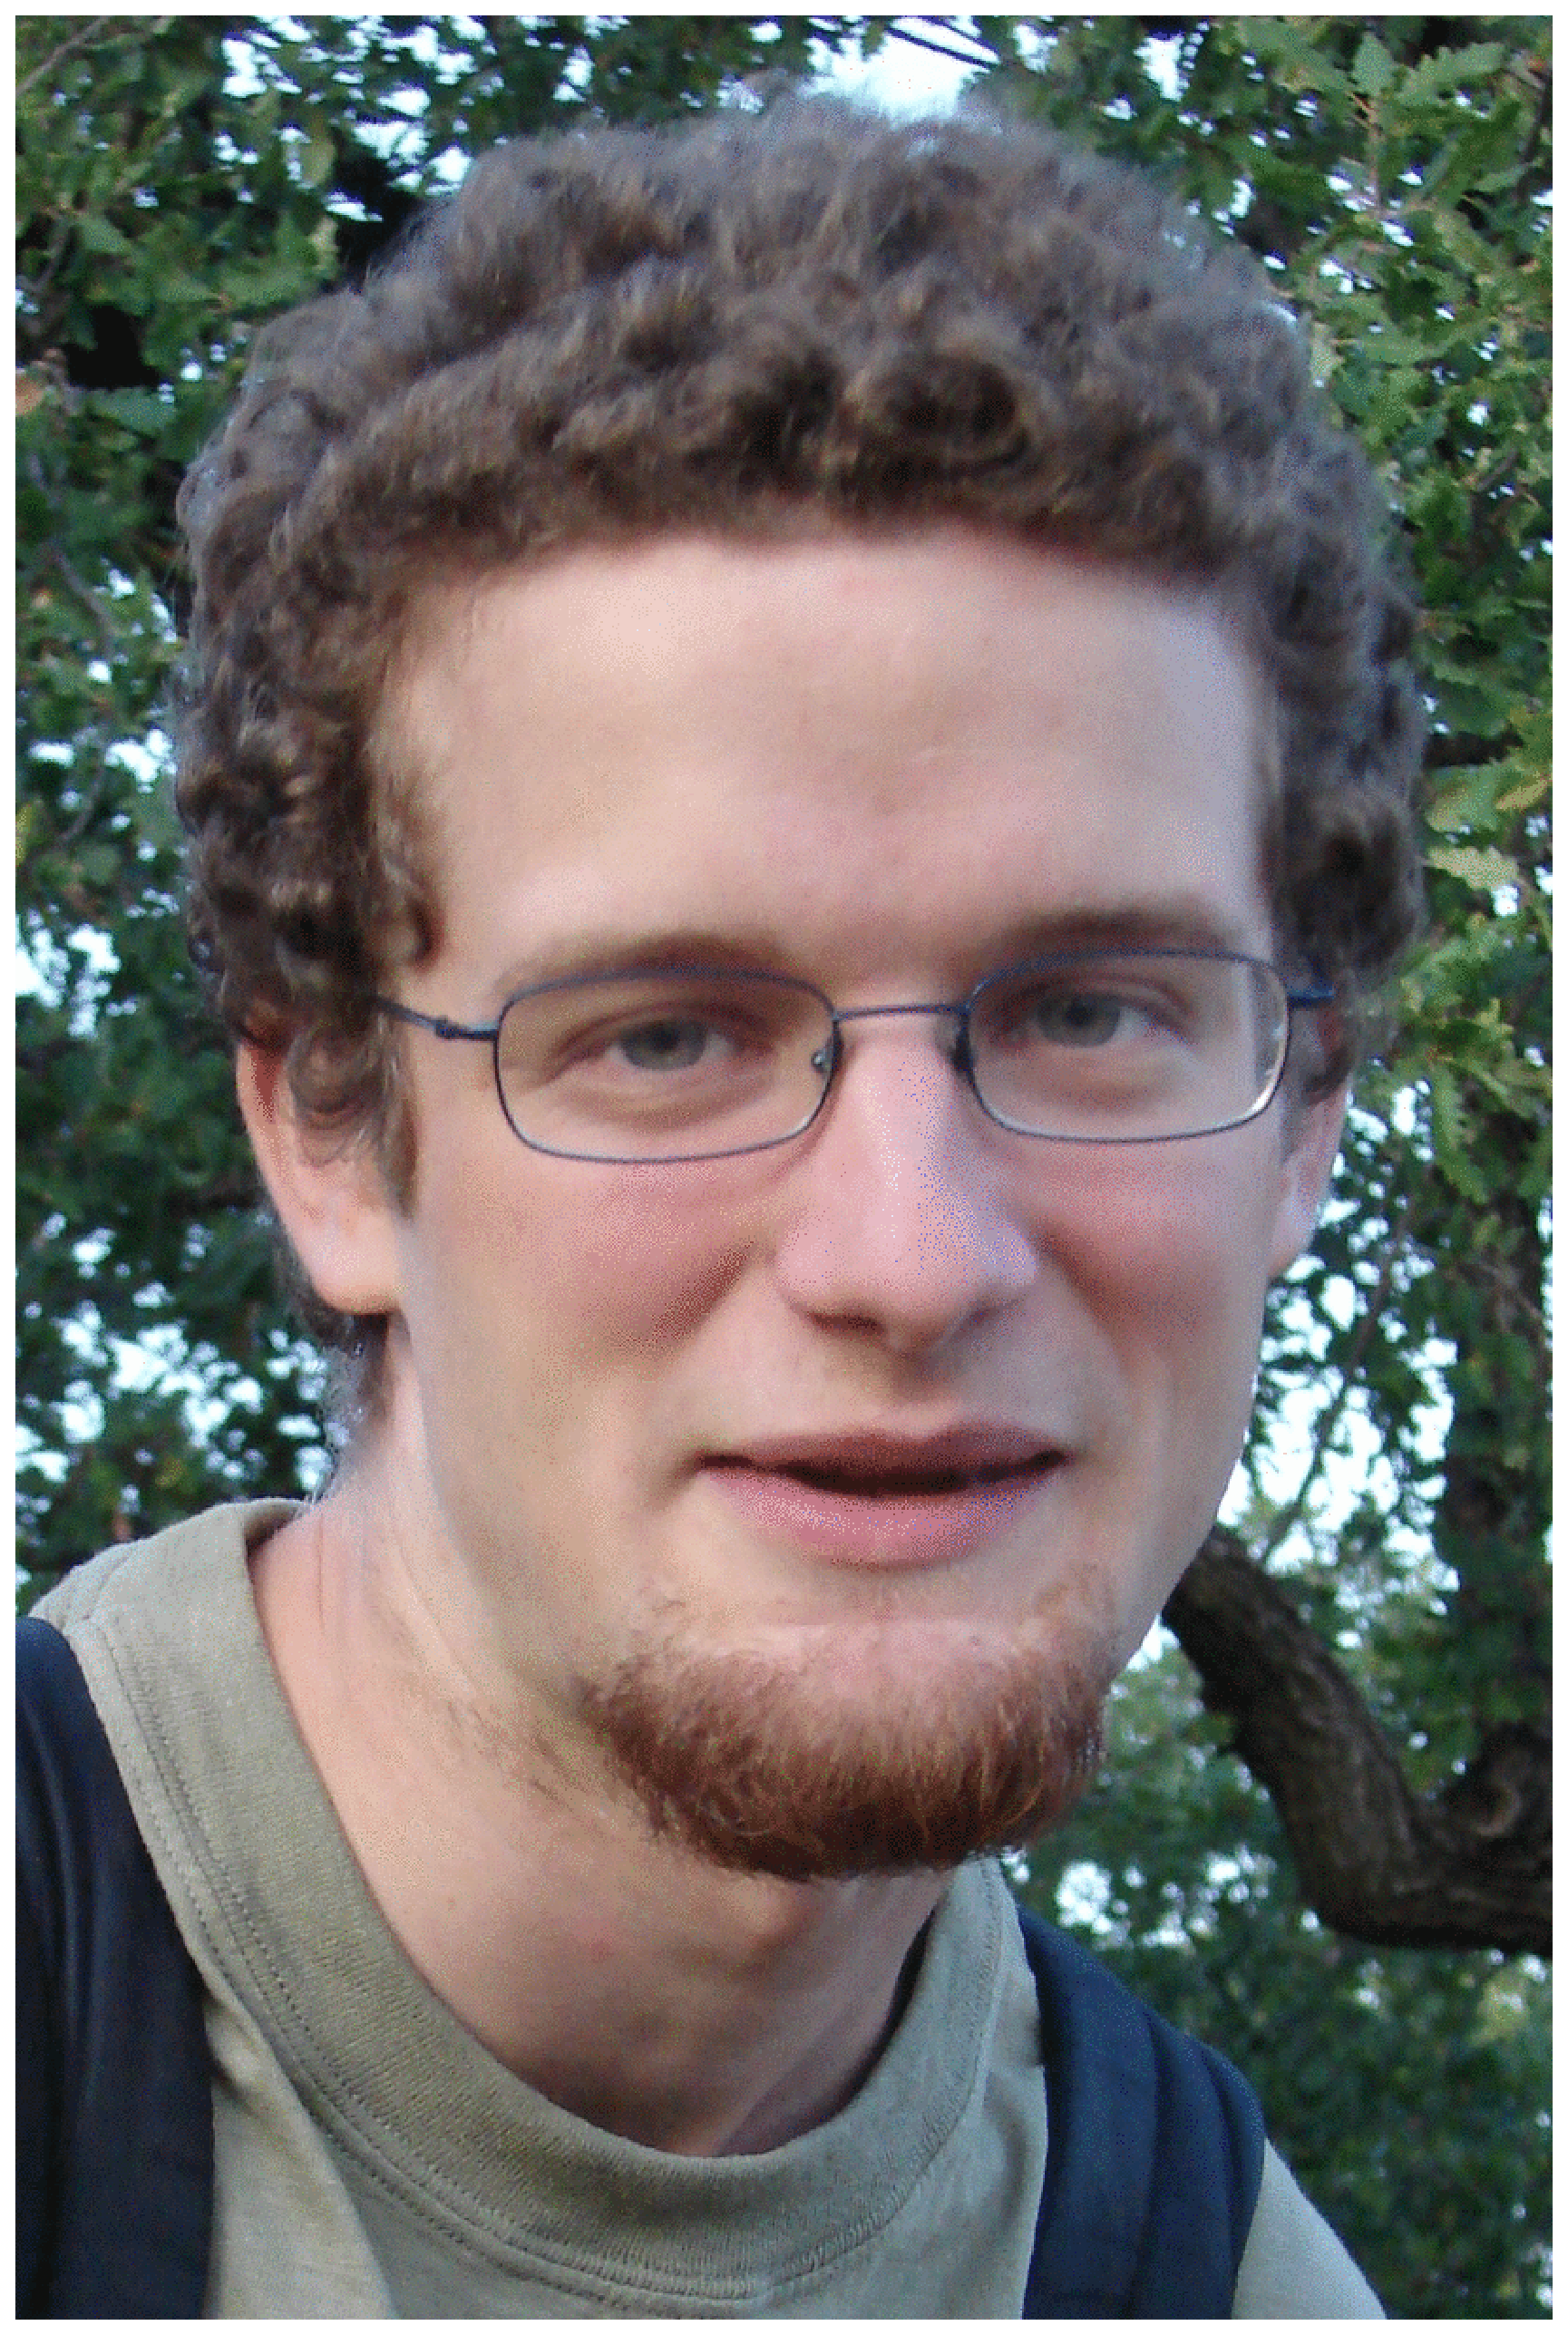
\includegraphics[width=20mm]{20090926.eps}} &
  \parbox{120mm}{
\begin{center}
\normalsize{Vajna Mikl�s (AYU9RZ),

2nd semester, (MSc) computer engineering student

Consultants: Dr. Szentiv�nyi G�bor, Dr. Sz�nt� Iv�n, ULX

Internal consultant: Horv�th �kos, MIT

Specialization in Dependable System Design

Project Laboratory 2 Interim Report

2010/11. 1st semester}
\end{center}
} \\
\end{tabular}


\end{center}
\thispagestyle{empty}
\newpage

\tableofcontents
\newpage

\section{Introduction}

The dm-mirror Linux kernel module is a software mirror implementation in the
Linux kernel, which is part of the device-mapper framework, most commonly used
for logical volume management (LVM\cite{lvm}).  The de facto common standard in industry
for software RAID in Linux environments is md-mirror nowadays, which is
independent from LVM.  My target is to improve dm-mirror in a way so that it's
feature set will be comparable (and then even better) to the already available
dm-mirror, while keeping it based on LVM.

My initial goal is to achieve fault tolerance and optimal performance in a
distributed storage setting with storage and network components having
different performance characteristics.

All my steps aim to converge the design and development dm-mirror in that
direction.

\section{Background}

Postponed: comparison of dm-mirror vs. md-mirror.

\section{The problems of dm-mirror}

My initial problem is that in a distributed environment the local and the
remote nodes have different characteristics and this should be supported when
accessing device nodes. For example, when reading, it's important to use the
fastest node available, or - a sightly fine-grained method - use a weighted
approach to read more from faster nodes. It's also important to tolerate and
handle failures in a proper way, since those happen a lot in distributed
systems.

Having a look at the current dm-mirror\cite{lvmmirror}, I saw:

\begin{itemize}
\item The current read method is a Round-Robin algorithm, which is not capable
of proper handling of device nodes with different read speed.
\item Fault tolerance is in its initial stage: when a device node fails and
later recovers, manual action is needed, which takes time.
\end{itemize}

\section{Implementation}

The LVM mirror consists of multiple legs: all but one serves as a data storage,
and one does logging. This way the storage part of the mirror can be
represented as an array of logical device nodes - in case of two data and one
mirror leg, there will be two elements in the array. We index it from zero, so
the first element will have an index 0, then the second data leg will have an
index 1. The default mirror is the leg which is currently currently used for
reading.

When I read the source code of dm-mirror, I found two problems which seemed to
be relatively easy to fix:

\begin{itemize}
\item In case the two legs of the mirror have different read access, it's a
good idea to completely disable the Round-Robin algorithm and read from the
default mirror only.
\item In case the default mirror is not the fastest one, the user will want to
set the default mirror to a non-zero index value.
\end{itemize}

The current behaviour is that a number of read operations are done on one
device, then a switch occurs. The switch is done exactly when a limit is
reached - this is called \emph{rr\_ios\_set} in the source code. This number has
to be greater or equal to one at the moment.
What I did is the following: I extended it to support zero as a value as well, and in that case a switch never occurs.

The kernel part of the support code is the following:

\begin{verbatim}
diff --git a/drivers/md/dm-raid1.c b/drivers/md/dm-raid1.c
index 23c1d65..0480708 100644
--- a/drivers/md/dm-raid1.c
+++ b/drivers/md/dm-raid1.c
@@ -849,6 +849,15 @@
   * the first we tried, so we know when we're done.
   */
  ret = start_mirror = ms->read_mirror;
+
+ /*
+  * If MIN_READS is zero, then always use the default one.
+  */
+       if (!atomic_read(&ms->rr_ios_set)) {
+         ret = ms->default_mirror;
+         goto use_mirror;
+       }
+
  do {
    if (likely(!atomic_read(&ret->error_count) &&
         !atomic_dec_and_test(&ms->rr_ios)))
@@ -1848,8 +1858,10 @@

  if (sscanf(argv[3], "%u", &rr_ios_set) != 1 ||
      rr_ios_set < 2) {
-         DMERR("Round robin read ios have to be > 1");
-         return -EINVAL;
+         if (rr_ios_set != 0) {
+           DMERR("Round robin read ios have to be > 1 or 0");
+           return -EINVAL;
+         }
  }

  md = dm_table_get_md(ti->table);
\end{verbatim}

And then the user-space command to disable the switches is the following:

\begin{verbatim}
# dmsetup message myvg-mymirror 0 \
    io_balance round_robin ios 0
\end{verbatim}

The first zero is the identifier of the device, the second one is the number
introducing the real change.

The second problem is about: once we disabled automatic switches, we want to set the default mirror manually. To allow this, I did the following modifications to the kernel part:

\begin{verbatim}
diff --git a/drivers/md/dm-raid1.c b/drivers/md/dm-raid1.c
index 0480708..47797a5 100644
--- a/drivers/md/dm-raid1.c
+++ b/drivers/md/dm-raid1.c
@@ -1846,31 +1846,47 @@
 /* Set round robin ios via message. */
 static int mirror_message(struct dm_target *ti,
                           unsigned argc, char **argv)
 {
-  unsigned rr_ios_set;
   struct mirror_set *ms = ti->private;
   struct mapped_device *md;
 
-  if (argc != 4 ||
-      strncmp(argv[0], "io_balance", strlen(argv[0])) ||
-      strncmp(argv[1], "round_robin", strlen(argv[1])) ||
-      strncmp(argv[2], "ios", strlen(argv[2])))
-    return -EINVAL;
-
-  if (sscanf(argv[3], "%u", &rr_ios_set) != 1 ||
-      rr_ios_set < 2) {
-    if (rr_ios_set != 0) {
-      DMERR("Round robin read ios have to be > 1 or 0");
-      return -EINVAL;
+  if (argc == 4 &&
+      !strncmp(argv[0], "io_balance", strlen(argv[0])) &&
+      !strncmp(argv[1], "round_robin", strlen(argv[1])) &&
+      !strncmp(argv[2], "ios", strlen(argv[2]))) {
+    unsigned rr_ios_set;
+    if (sscanf(argv[3], "%u", &rr_ios_set) != 1 ||
+        rr_ios_set < 2) {
+      if (rr_ios_set != 0) {
+        DMERR("Round robin read ios have to be > 1 or 0");
+        return -EINVAL;
+      }
     }
+
+    md = dm_table_get_md(ti->table);
+    DMINFO("Setting round robin read ios for \"%s\" to %u",
+        dm_device_name(md), rr_ios_set);
+    dm_put(md);
+    atomic_set(&ms->rr_ios_set, rr_ios_set);
+    atomic_set(&ms->rr_ios, rr_ios_set);
+    return 0;
   }
 
-  md = dm_table_get_md(ti->table);
-  DMINFO("Setting round robin read ios for \"%s\" to %u",
-          dm_device_name(md), rr_ios_set);
-  dm_put(md);
-  atomic_set(&ms->rr_ios_set, rr_ios_set);
-  atomic_set(&ms->rr_ios, rr_ios_set);
-  return 0;
+  if (argc == 3 &&
+    !strncmp(argv[0], "io_balance", strlen(argv[0])) &&
+    !strncmp(argv[1], "default", strlen(argv[1]))) {
+    unsigned int m;
+    for (m = 0; m < ms->nr_mirrors; m++)
+      if (!strncmp(argv[2], ms->mirror[m].dev->name,
+                   strlen(argv[2]))) {
+        ms->default_mirror = &ms->mirror[m];
+        md = dm_table_get_md(ti->table);
+        DMINFO("Setting default device for \"%s\" to \"%s\"",
+            dm_device_name(md), argv[2]);
+        dm_put(md);
+        return 0;
+      }
+  }
+
+  return -EINVAL;
 }
 
 /*
\end{verbatim}

The user-space setting then can be used as follows:

\begin{itemize}
\item Use \emph{lvs -a -o +devices} to list devices, the \emph{mimage} nodes will be the physical nodes of a mirror.
\item Once you have the right mimage, use \emph{dmsetup ls} to get the real device number, for example 253:3.
\item Finally use \emph{dmsetup message} to send the wished device number to the kernel
\end{itemize}

A possible commandline is:

\begin{verbatim}
# dmsetup message myvg-mymirror 0 io_balance default 253:3
\end{verbatim}

\section{Measurements}

I used the following setup for the tests:

\begin{figure}[H]
\centering
\includegraphics[width=150mm,keepaspectratio]{testarch.eps}
\caption{Architecture of the test environment}
\end{figure}

The two machines were virtual ones, projlab2 hosted the LVM mirror, I ran all
timers there, finally that was the iSCSI initiator. The other box served as the
iSCSI target. Additionally I limited the bandwidth there, and I added the
network delay there as well.

I had two scripts to limit bandwidth and to add network delay to the traffic of
the iSCSI target.

The network delay part is more simple. To add some delay to each outgoing or
incoming package on the \emph{eth0} interface, the \emph{tc} command can be
used:

\begin{verbatim}
tc qdisc add dev eth0 root netem delay 100ms
\end{verbatim}

In case the delay is no longer necessary, a single command can remove the above
rule:

\begin{verbatim}
tc qdisc del dev eth0 root
\end{verbatim}

The Linux Advanced Routing and Traffic Control HOWTO\cite{lartc} explains the
\emph{tc} command in more detail.

There are multiple ways to limit bandwidth. And older technique is Class Based
Queueing, a newer one is Hierarchy Token Bucket. In short, HTB is a successor
to CBQ, see its documentation\cite{htb} fore more details.

The LARC HOWTO even provides a ready to use script to limit bandwidth, I used
that without any major modifications.

\subsection{Read speed}

First I checked the read time of a 2MB-sized file without network latency and
with 200ms delay over an iSCSI device node. I following table and chart
demonstrate the results (all numbers are in seconds, unless otherwise stated):

\begin{center}
\begin{table}[H]
\centering
\begin{tabular}{| l | l |}
\hline
Type & Time \\ \hline
Local read & 0.03 \\
Remote read & 17.642 \\
\hline
\end{tabular}
\caption{Local and remote reads with network latency}
\end{table}
\end{center}

\begin{figure}[H]
\centering
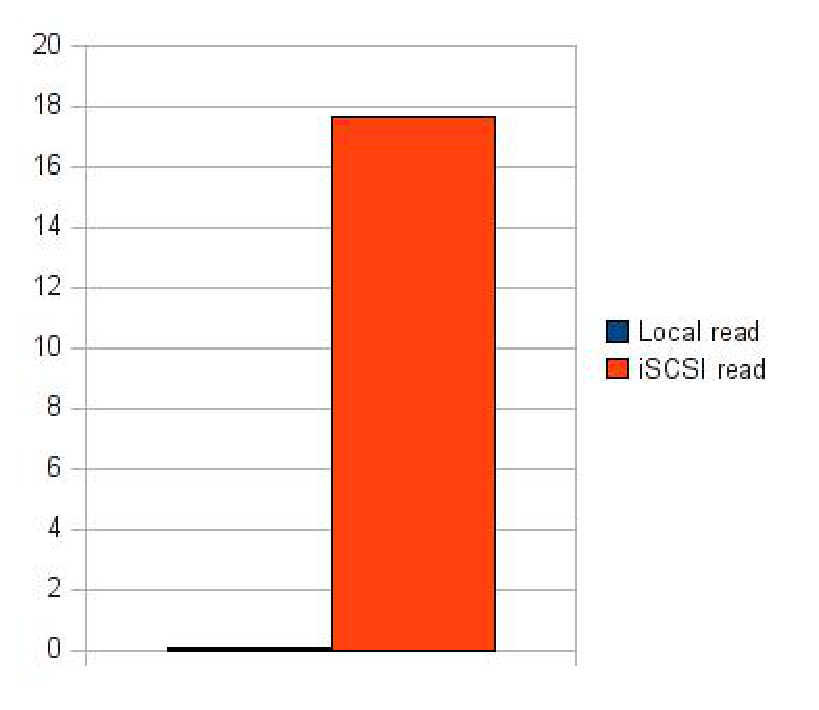
\includegraphics[width=75mm,keepaspectratio]{charts/1_63947f00.eps}
\caption{Comparing local and remote reads with network latency}
\end{figure}

The reason for such a huge difference with 200ms latency is that this delay is
meant for each package, while the transferred data is 2MB.

Then I measured read speed of 2MB data on a mirror (every result is the average
of 3 individual measures):

\begin{center}
\begin{table}[H]
\centering
\begin{tabular}{| l | l |}
\hline
Type & Time \\ \hline
Default (RR, n=128) with delay & 3.598 \\
Local only & 0.255 \\
Remote without delay & 1.636 \\
Remote with delay & 18.796 \\
\hline
\end{tabular}
\caption{Mirror read speed of 2MB data}
\end{table}
\end{center}

\begin{figure}[H]
\centering
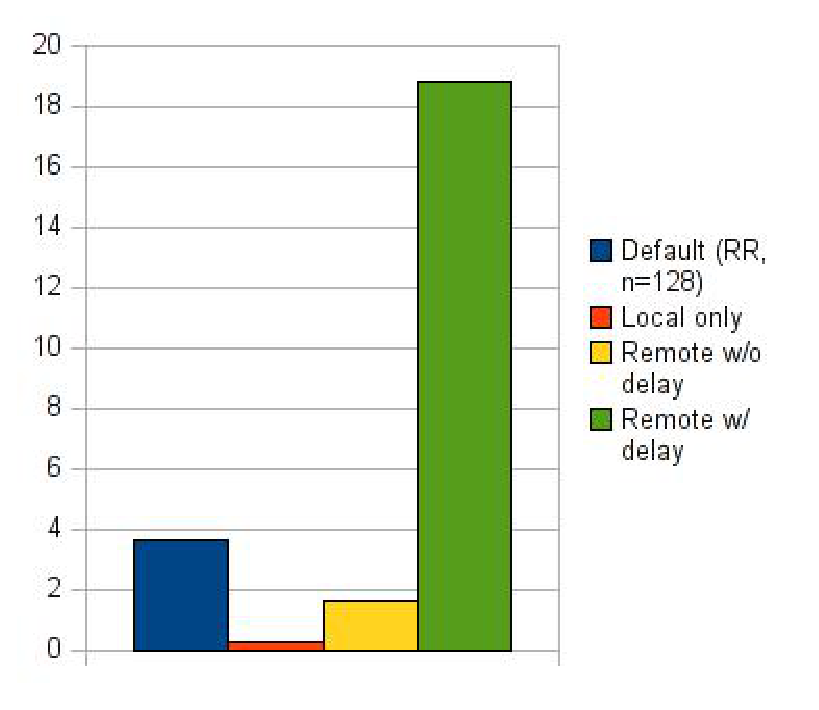
\includegraphics[width=75mm,keepaspectratio]{charts/7_69a4ab34.eps}
\caption{Comparing mirror read speed of 2MB data}
\end{figure}

As expected, the fastest method is doing all reads on the local node exclusively.

By remote "with" or "without" delay, I mean that in the first situation I used
the \emph{tc} tool to add some simulated delay, while in the second case I
didn't use such a tool, so basically there were no delay. (Because the two
virtual machines were on the same physical host.)

It makes sense to calculate if the results are approximately valid before we
continue. The total delay of packages from the above table is 17.160s. If the
delay for each logical package is 200ms, that should mean about 86 logical
packages. By logical, I mean I don't count physical fragmentation of the IP
packages.  When I recorded the network traffic with \emph{tcpdump}, then I got
70 packages having the TCP PUSH flag (last physical IP package of a logical
write). The difference is measure error, we already saw above that the result
varies a bit each time we repeat the test. As a result, sadly it's not entirely
possible to exactly repeat the same test with and without network delay.

Now that we understand the difference between remote reads with and without
network delay, let's compare the other results. Reading using Round Robin (with
delay) is slower than a remote read without delay, we expected that. Also,
reading from remote with delay is slower than reading from local and remote
(what RR does) as well, so the results show what we would predict.

\subsection{Write speed}

First I measured write speed with different network bandwidth available. In this case no LVM technique was involved, I used plain scp to copy data projlab2 to iscsitarget:

\begin{center}
\begin{table}[H]
\centering
\begin{tabular}{| l | l |}
\hline
Type & Time \\ \hline
10kbit & 22.951 \\
100mbit & 1.705 \\
unlimited & 1.767 \\
\hline
\end{tabular}
\caption{Network write speed with 2MB of data}
\end{table}
\end{center}

\begin{figure}[H]
\centering
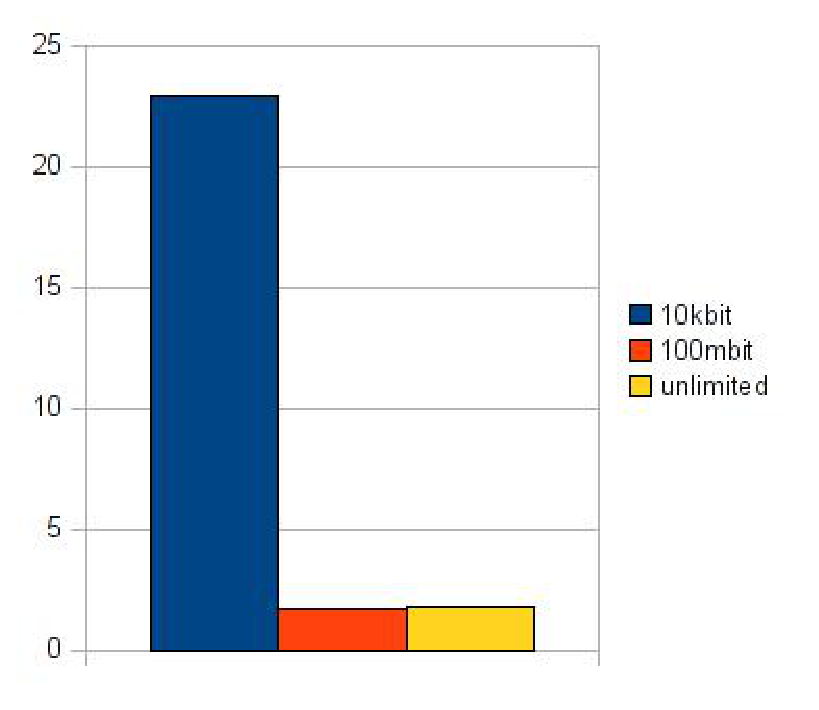
\includegraphics[width=75mm,keepaspectratio]{charts/2_5fabe87e.eps}
\caption{Comparing network write speed with 2MB of data}
\end{figure}

From now, I measured mirror write speed of 2MB data, with various parameters.

\subsubsection{Singe log, local log, local disks}

Setup:

\begin{verbatim}
[root@projlab2 ~]# vgcreate myvg /dev/sdb /dev/sdc /dev/sdd
  Volume group "myvg" successfully created
[root@projlab2 ~]# lvcreate -L 900M -n mymirror -m 1 myvg
  Logical volume "mymirror" created
[root@projlab2 ~]# mke2fs -j /dev/myvg/mymirror
\end{verbatim}

\begin{figure}[H]
\centering
\includegraphics[width=75mm,keepaspectratio]{setup1.eps}
\caption{Architecture of single log, local log, local disks}
\end{figure}

That is a single measurement (3 times, and then counting the average in seconds):
0.594.

Tear down:

\begin{verbatim}
[root@projlab2 ~]# lvchange -a n myvg/mymirror
[root@projlab2 ~]# lvremove myvg/mymirror
  Logical volume "mymirror" successfully removed
[root@projlab2 ~]# vgremove myvg
  Volume group "myvg" successfully removed
\end{verbatim}

\subsubsection{Single log, remote log, local and remote disk, different ratios}

Setup: I created sdb1 and sdb1 on iscsitarget and started the daemon:

\begin{verbatim}
[root@iscsitarget ~]# /etc/init.d/tgtd start
Starting SCSI target daemon: [  OK  ]
\end{verbatim}

Then I configured the client:

\begin{verbatim}
[root@projlab2 ~]# /etc/init.d/iscsi start
iscsid (pid  2237) is running...
Setting up iSCSI targets: Logging in to
 [iface: default, target: iqn.2008-03.local.virtual2:storage,
 portal: 192.168.152.130,3260]
Login to [iface: default,
 target: iqn.2008-03.local.virtual2:storage,
 portal: 192.168.152.130,3260]: successful
 [  OK  ]
[root@projlab2 ~]# fdisk -l|tail -n 2
/dev/sdf1               1          65      522081   83  Linux
/dev/sdf2              66         130      522112+  83  Linux
\end{verbatim}

As you can see above, the remote disk appeared as sdf. Finally I configured the mirror:

\begin{verbatim}
[root@projlab2 ~]# vgcreate myvg /dev/sdb /dev/sdf1 /dev/sdf2
  Volume group "myvg" successfully created
[root@projlab2 ~]# lvcreate -L 400M -n mymirror -m 1 myvg
  Logical volume "mymirror" created
[root@projlab2 ~]# tail -n 1 /var/log/messages
Oct  6 20:50:36 projlab2 lvm[3487]:
 myvg-mymirror is now in-sync.
[root@projlab2 ~]# mke2fs -j /dev/myvg/mymirror
\end{verbatim}

\begin{figure}[H]
\centering
\includegraphics[width=150mm,keepaspectratio]{setup2.eps}
\caption{Architecture of single log, remote log, local and remote disks}
\end{figure}

\begin{center}
\begin{table}[H]
\centering
\begin{tabular}{| l | l |}
\hline
Type & Time \\ \hline
1:2 & 1.828 \\
1:5 & 22.872 \\
1:10 & 37.621 \\
1:50 & 47.642 \\
1:100 & 48.643 \\
\hline
\end{tabular}
\caption{Network write speed with single log, remote log, local and remote disk, different ratios}
\end{table}
\end{center}

\begin{figure}[H]
\centering
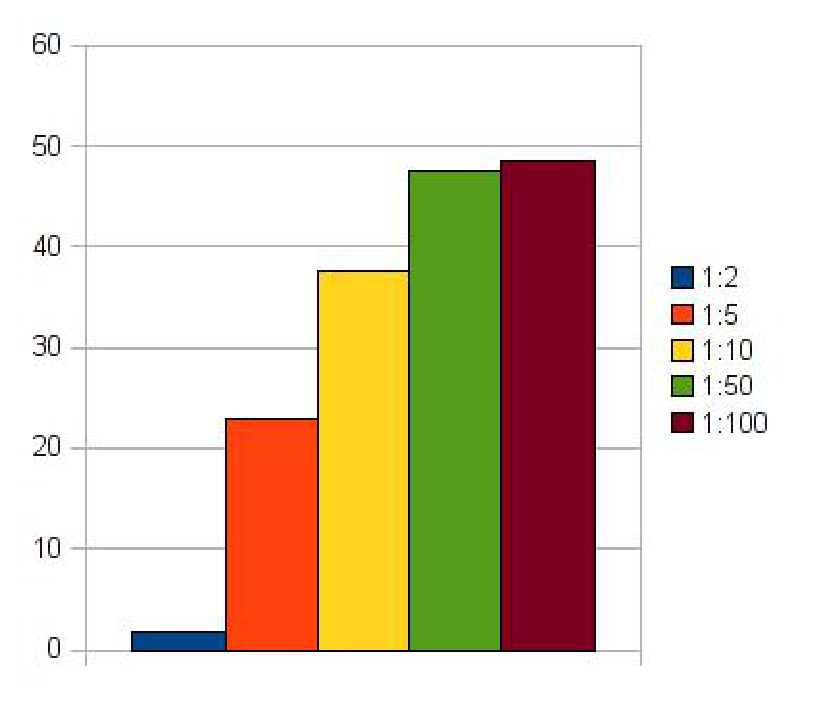
\includegraphics[width=75mm,keepaspectratio]{charts/3_5e6daa6.eps}
\caption{Comparing network write speed with single log, remote log, local and remote disk, different ratios}
\end{figure}

Tear down: I disabled bandwith limitation.

\subsubsection{Single log, remote log, local and remote disk, different delays}

No setup, the mirror was already there.

\begin{center}
\begin{table}[H]
\centering
\begin{tabular}{| l | l |}
\hline
Type & Time \\ \hline
5ms & 0.823 \\
10ms & 0.752 \\
50ms & 2.676 \\
100ms & 4.341 \\
200ms & 13.558 \\
\hline
\end{tabular}
\caption{Network write speed with single log, remote log, local and remote disk, different delays}
\end{table}
\end{center}

\begin{figure}[H]
\centering
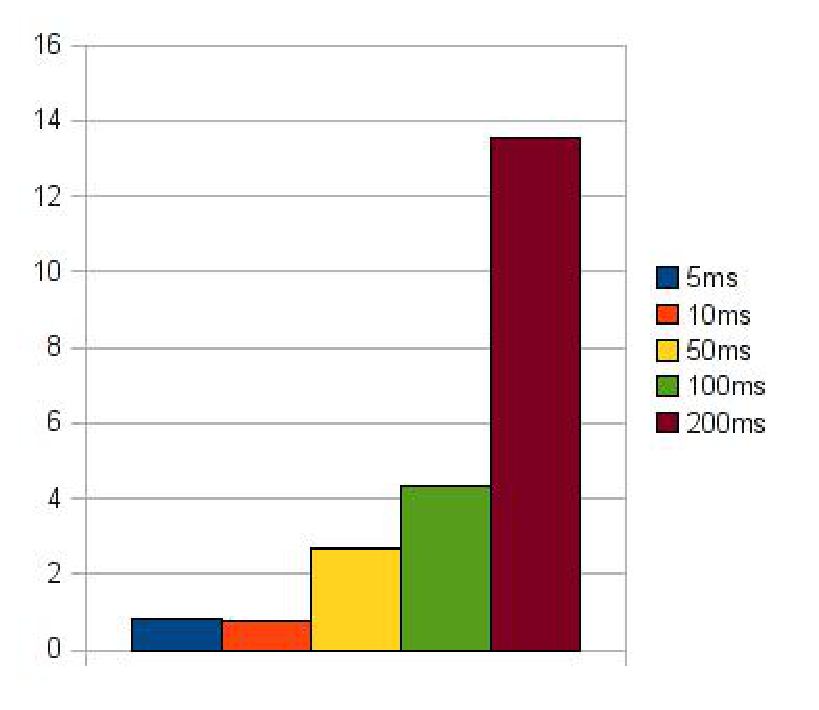
\includegraphics[width=75mm,keepaspectratio]{charts/4_m724ff87b.eps}
\caption{Comparing network write speed with single log, remote log, local and remote disk, different delays}
\end{figure}

Tear down: I disabled the simulation of network latency, then:

\begin{verbatim}
[root@iscsitarget ~]# ./delay.sh stop
[root@projlab2 ~]# lvchange -a n myvg/mymirror
[root@projlab2 ~]# lvremove myvg/mymirror
  Logical volume "mymirror" successfully removed
[root@projlab2 ~]# vgremove myvg
  Volume group "myvg" successfully removed
\end{verbatim}

\subsubsection{Single log, local log, local and remote disk, different ratios}

Set up:

\begin{verbatim}
[root@projlab2 ~]# vgcreate myvg /dev/sdb /dev/sdf1 /dev/sdc
  Volume group "myvg" successfully created
[root@projlab2 ~]# lvcreate -L 400M -n mymirror -m 1 myvg
  Logical volume "mymirror" created
[root@projlab2 ~]# tail -n 1 /var/log/messages
Oct  6 21:25:18 projlab2 lvm[3487]:
 myvg-mymirror is now in-sync.
[root@projlab2 ~]# mke2fs -j /dev/myvg/mymirror
\end{verbatim}

\begin{figure}[H]
\centering
\includegraphics[width=150mm,keepaspectratio]{setup3.eps}
\caption{Architecture of single log, local log, local and remote disks}
\end{figure}

\begin{center}
\begin{table}[H]
\centering
\begin{tabular}{| l | l |}
\hline
Type & Time \\ \hline
1:2 & 3.384 \\
1:5 & 7.032 \\
1:10 & 6.876 \\
1:50 & 45.978 \\
1:100 & 47.815 \\
\hline
\end{tabular}
\caption{Network write speed with single log, local log, local and remote disk, different ratios}
\end{table}
\end{center}

\begin{figure}[H]
\centering
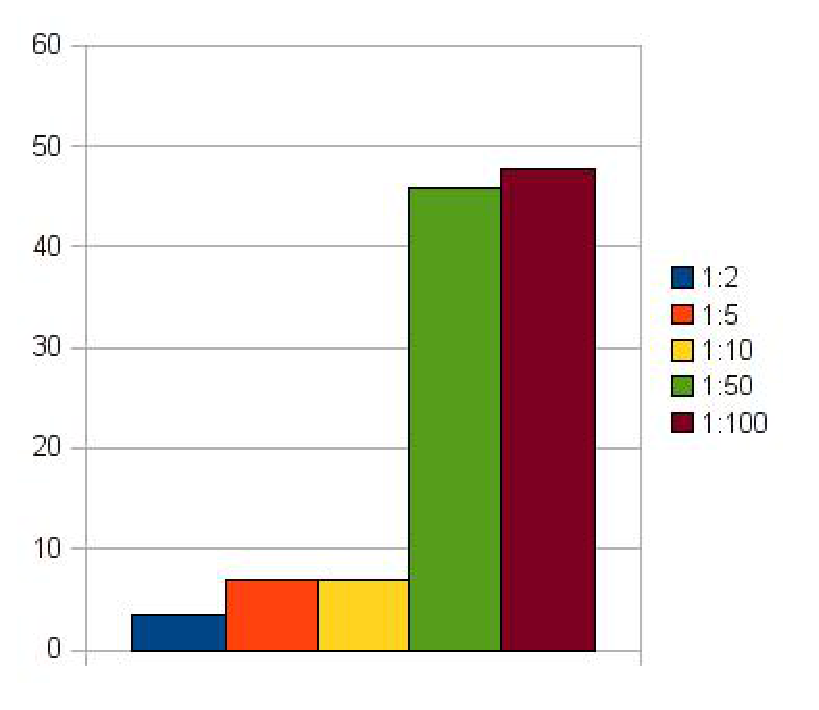
\includegraphics[width=75mm,keepaspectratio]{charts/5_5d601c11.eps}
\caption{Comparing network write speed with single log, local log, local and remote disk, different ratios}
\end{figure}

Tear down: I disabled bandwidth limitation.

\subsubsection{Single log, local log, local and remote disk, different delays}

No setup, the mirror is the same as with the previous test.

\begin{center}
\begin{table}[H]
\centering
\begin{tabular}{| l | l |}
\hline
Type & Time \\ \hline
5ms & 3.463 \\
10ms & 3.328 \\
50ms & 3.026 \\
100ms & 4.762 \\
200ms & 7.337 \\
\hline
\end{tabular}
\caption{Network write speed with single log, local log, local and remote disk, different delays}
\end{table}
\end{center}

\begin{figure}[H]
\centering
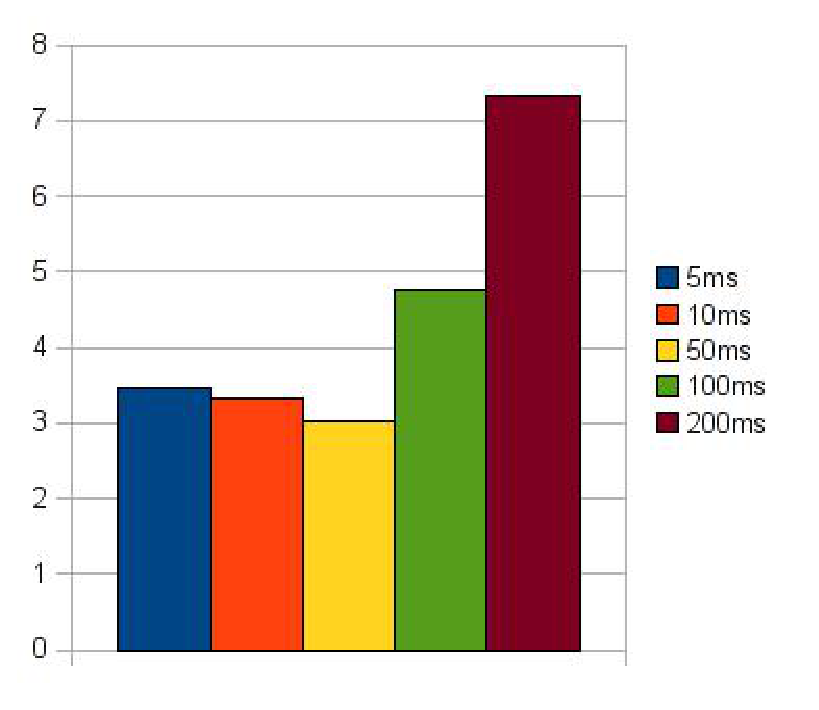
\includegraphics[width=75mm,keepaspectratio]{charts/6_273f2c73.eps}
\caption{Comparing network write speed with single log, local log, local and remote disk, different delays}
\end{figure}

Tear down: I disabled network latency, then:

\begin{verbatim}
[root@projlab2 ~]# lvchange -a n myvg/mymirror
[root@projlab2 ~]# lvremove myvg/mymirror
  Logical volume "mymirror" successfully removed
[root@projlab2 ~]# vgremove myvg
  Volume group "myvg" successfully removed
\end{verbatim}

\subsubsection{Mirrored log, local disks}

For now, I tested this on my RHEL5 machine where I already had the backported
lvm2 from Fedora rawhide. This has the benefit that other components of the system
is not changed. The downside is that this way the measurement is less official,
since then this is a custom system.

Set up:

\begin{verbatim}
[root@projlab2 ~]# vgcreate myvg \
  /dev/sdb /dev/sdc /dev/sdd /dev/sde
  Volume group "myvg" successfully created
[root@projlab2 ~]# lvcreate -L 400M -n mymirror -m 1 myvg \
  --mirrorlog mirrored
  Logical volume "mymirror" created
[root@projlab2 ~]# mke2fs -j /dev/myvg/mymirror 
\end{verbatim}

\begin{figure}[H]
\centering
\includegraphics[width=75mm,keepaspectratio]{setup4.eps}
\caption{Architecture of mirrored log, local disks}
\end{figure}

That is a single measurement (3 times, and then counting the average in seconds):
3.186.

Tear down:

\begin{verbatim}
[root@projlab2 ~]# lvchange -a n myvg/mymirror
[root@projlab2 ~]# lvremove myvg/mymirror
  Logical volume "mymirror" successfully removed
[root@projlab2 ~]# vgremove myvg
  Volume group "myvg" successfully removed
\end{verbatim}

\subsubsection{Mirrored log, local and remote disk, different ratios}

Set up:

\begin{verbatim}
[root@projlab2 ~]# vgcreate myvg \
  /dev/sdb /dev/sdf1 /dev/sdc /dev/sdf2
  Volume group "myvg" successfully created
[root@projlab2 ~]# lvcreate -L 400M -n mymirror -m 1 myvg \
  --mirrorlog mirrored
  Logical volume "mymirror" created
[root@projlab2 ~]# tail -n 1 /var/log/messages
Oct  6 22:08:58 projlab2 lvm[3487]:
 myvg-mymirror is now in-sync.
[root@projlab2 ~]# mke2fs -j /dev/myvg/mymirror
\end{verbatim}

\begin{figure}[H]
\centering
\includegraphics[width=150mm,keepaspectratio]{setup5.eps}
\caption{Architecture of mirrored log, local and remote disks}
\end{figure}

\begin{center}
\begin{table}[H]
\centering
\begin{tabular}{| l | l |}
\hline
Type & Time \\ \hline
1:2 & 2.032 \\
1:5 & 22.661 \\
1:10 & 38.246 \\
1:50 & 47.09 \\
1:100 & 49.026 \\
\hline
\end{tabular}
\caption{Network write speed with mirrored log, local and remote disk, different ratios}
\end{table}
\end{center}

\begin{figure}[H]
\centering
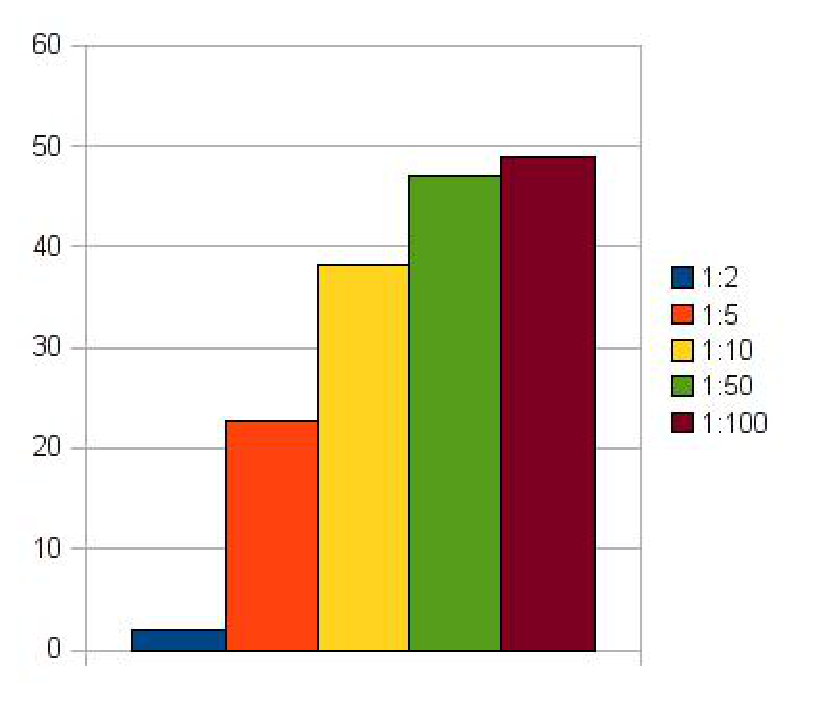
\includegraphics[width=75mm,keepaspectratio]{charts/8_m1d51a4a2.eps}
\caption{Comparing network write speed with mirrored log, local and remote disk, different ratios}
\end{figure}

Tear down: I stopped the bandwith limit.

\subsubsection{Mirrored log, local and remote disk, different delays}

No setup, I re-used the mirror from the previous test.

\begin{center}
\begin{table}[H]
\centering
\begin{tabular}{| l | l |}
\hline
Type & Time \\ \hline
5ms & 0.946 \\
10ms & 0.939 \\
50ms & 3.222 \\
100ms & 5.175 \\
200ms & 12.384 \\
\hline
\end{tabular}
\caption{Network write speed with mirrored log, local and remote disk, different delays}
\end{table}
\end{center}

\begin{figure}[H]
\centering
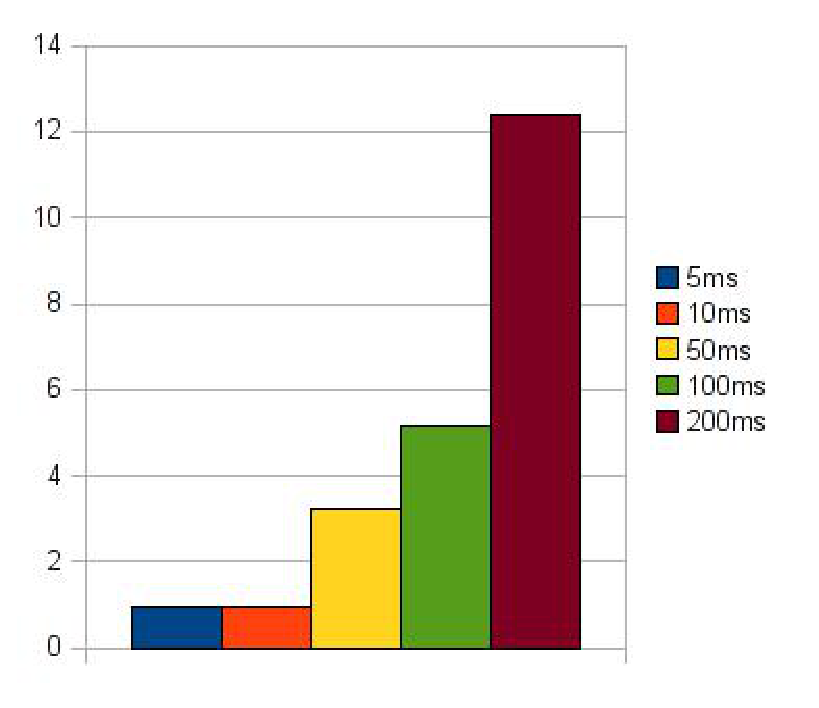
\includegraphics[width=75mm,keepaspectratio]{charts/9.eps}
\caption{Comparing network write speed with mirrored log, local and remote disk, different delays}
\end{figure}

Tear down: I disabled network latency, then:

\begin{verbatim}
[root@projlab2 ~]# lvchange -a n myvg/mymirror
[root@projlab2 ~]# lvremove myvg/mymirror
  Logical volume "mymirror" successfully removed
[root@projlab2 ~]# vgremove myvg
  Volume group "myvg" successfully removed
[root@projlab2 ~]# /etc/init.d/iscsi stop
Logging out of session [sid: 1, target:
 iqn.2008-03.local.virtual2:storage,
 portal: 192.168.152.130,3260]
Logout of [sid: 1,
 target: iqn.2008-03.local.virtual2:storage,
 portal: 192.168.152.130,3260]: successful
Stopping iSCSI daemon: 
[root@projlab2 ~]# ls /dev/sdf
ls: /dev/sdf: No such file or directory
\end{verbatim}

\subsection{Conclusions}

\begin{itemize}
\item The measured numbers are not always the ones we expected, though generally they are OK, I think.
\item One false effect is that \emph{sync} does not do empty the write cache on the \emph{iscsitarget} (remote) node.
\item In general, I would say the mirrored log is a nice feature, as that way
the two leg of the mirror can be really identical.

On the other hand, it seems to be a huge overhead. This means that in case
dm-mirror is running on one machine only, it is not a major benefit. This is
because in case dm-mirror has a single local log, that's already enough.

Note: dm-mirror is running on multiple boxes in cluster environments, so it
still makes sense to have mirrored logs in those cases.
\end{itemize}

\section{What to work on next}

I basically have three ideas on where could I continue:

\begin{itemize}
\item Even though I already did some measurement, more could be necessary. Maybe a more automated setup would provide better numbers. The current measures were executed manually, then I had to copy the numbers to this document, finally I manually created the charts as well. This may worth more automatism.
\item I could do further research on how to improve performance. For example it would be possible to let the dm-mirror kernel module handle do weighted RR, in case a simple RR is suboptimal, but reading from a single disk only isn't the best, either.
\item Finally, sooner or later it will be important to add support for storing the RR number and the default mirror device in the LVM metadata.
\end{itemize}

If it's up to me, I would say the last one is the more interesting, since
currently the dmsetup commands have to be put to some init script which is
executed on startup any time, which is a bit ugly.

%\clearpage

\begin{thebibliography}{4}
\addcontentsline{toc}{section}{References}

\bibitem{lvm} Logical Volume Manager 2, http://sources.redhat.com/lvm2/
\bibitem{lvmmirror} Mirror Volumes Using Logical Volume Manager, RedHat Enterprise Linux 5 \\ Documentation, \url{http://bit.ly/bkcn6d}
\bibitem{lartc} Linux Advanced Routing and Traffic Control HOWTO, http://lartc.org/howto/index.html
\bibitem{htb} Hierarchy Token Bucket qdisc in Linux, http://lartc.org/manpages/tc-htb.html

\end{thebibliography}
\end{document}
